%Input preamble
%Style
\documentclass[11pt]{article}
\usepackage[top=1in, bottom=1in, left=1in, right=1in]{geometry}
\parindent 22pt

%Packages
\usepackage{amsmath}
\usepackage{amsfonts}
\usepackage{amssymb}
\usepackage{bm}
\usepackage[table]{xcolor}
\usepackage{tabu}
\usepackage{makecell}
\usepackage{longtable}
\usepackage{multirow}
\usepackage[normalem]{ulem}
\usepackage{etoolbox}
\usepackage{graphicx}
\usepackage{tabularx}
\usepackage{ragged2e} 
\usepackage{booktabs}
\usepackage{caption}
\usepackage[none]{hyphenat}
\usepackage{fixltx2e}
\usepackage{threeparttablex}
\usepackage[capposition=top]{floatrow}
\usepackage{subcaption}
\usepackage{pdfpages}
\usepackage{pdflscape}
\usepackage{natbib}
\definecolor{maroon}{HTML}{990012}
\usepackage[colorlinks=true,linkcolor=maroon,citecolor=maroon]{hyperref}
\usepackage{tikz}
\usetikzlibrary{shapes}
\usepackage{setspace}

%Functions
\DeclareMathOperator{\cov}{Cov}
\DeclareMathOperator{\var}{Var}
\DeclareMathOperator{\plim}{plim}
\DeclareMathOperator{\Emax}{Emax}

%Math Environments
\newtheorem{theorem}{Theorem}[section]
\newtheorem{claim}[theorem]{Claim}
\newtheorem{assumption}[theorem]{Assumption}
\newtheorem{definition}[theorem]{Definition}
\newtheorem{hypothesis}[theorem]{Hypothesis}
\newtheorem{property}[theorem]{Property}
\newtheorem{example}[theorem]{Example}
\newtheorem{condition}[theorem]{Condition}
\newtheorem{exercise}[theorem]{Exercise}
\newtheorem{remark}[theorem]{Remark}
\newenvironment{proof}{\paragraph{Proof:}}{\hfill$\square$}

%Commands
\newcommand\independent{\protect\mathpalette{\protect\independenT}{\perp}}
\def\independenT#1#2{\mathrel{\rlap{$#1#2$}\mkern2mu{#1#2}}}
\newcommand{\overbar}[1]{\mkern 1.5mu\overline{\mkern-1.5mu#1\mkern-1.5mu}\mkern 1.5mu}
\newcommand{\equald}{\ensuremath{\overset{d}{=}}}

%Logo
\AddToShipoutPictureBG{%
  \AtPageUpperLeft{\raisebox{-\height}{
\includegraphics[width=1.5cm]{uchicago.png}}}
}




\begin{document}

\title{\textbf{Structural Econometrics with Implementations in Julia}}
\author{Jorge Luis Garc\'{i}a\thanks{Department of Economics, the University of Chicago (jorgelgarcia@uchicago.edu).} $^{,}$\thanks{A rough version of this document with an implementation in Python was delivered as an assignment when we were TAs for Econ 350 at the University of Chicago. We developed it together with Yike Wang, who we thank for many useful comments.}}
\date{First Draft: June 1, 2014 \\ This Draft: \today}
\maketitle

\begin{abstract}
\noindent This document briefly describes what are structural models in Economics. It distinguishes structural and non-structural estimation as approaches that enable to answer different research questions. Also, it discusses parametric and non-parametric assumptions as auxiliary means that help to recover parameters enabling to answer these research questions. The document builds on \citet{keane2011structural}. The difference between this document and that paper is that this document intends to be more concrete and schematic about how the modeling approaches behave, it skips the least algebra steps in all the derivations, and it provides practical examples. Finally, it provides extra exercises teaching basic tools of Computational Econometrics and implements them in Julia. Almost all of the implementations are available in Python as well, for the sake of language and efficiency comparison.
\end{abstract}

%Input Sections
\section{Introduction} \label{section:intro}
\noindent The objective of this document is to build on \citet{keane2011structural} and clarify Structural Estimation methods and its computational implementations. The focus is on the estimation of Discrete Choice Dynamic Programming (DCDP) models. In particular, the idea is to (i) illustrate the basic ideas and concepts; (ii) provide examples; (iii) become familiar with computational methods.\\

\subsection{DCDP as an Extension of the Static Discrete Choice Framework} \label{section:extension}
DCDP models are a natural generalization of static discrete choice models. They share the latent variable specification. To illustrate this, consider a binary choice model in which an economic agent, $i$, makes a choice at each discrete period $t$. $\mathcal{I}$ indexes individuals and $\mathcal{T}$ time. She has two alternatives: $d_{it} \in \{ 0,1\}$. A latent variable, $v_{it}^*$, which is the difference in the expected payoffs between the choices $d_{it} = 1$ and $d_{it} = 0$, determines the outcome. Specifically, if $v_{it}^*$ is greater than certain threshold, the agent chooses $d_{it} = 1$. Without loss of generality, the threshold is normalized to zero. Thus, $d_{it} = 1$ iff $v_{it}^* \geq 0$ and $d_{it} = 0$ otherwise.\\
\begin{exercise} (Identification of the Probit Model) \label{exercise:idenprobit}
Model a bivariate, static, discrete choice through a Probit model. The convention is that in this model the unobserved variable is normally distributed. (i) Show that you can normalize the threshold that defines the agent's decision without loss of generality;  (ii) why is the normalization without loss of generality?; (iii) what other normalization can you make without loss of generality in your Probit model?; (iv) what does this normalization implies with respect to the distribution of the unobserved variable? (v) are you able to identify all the parameters of the model?; (vi) how does identification and the normalizations relate to each other? Hint: think of the scalar and spatial identification issues that the structure of a Probit model generates.\\
\noindent Answer:\\
\noindent See the separate handout. 
\end{exercise}

\begin{exercise} (Computational Econometrics: Warm-up)
Solve the exercise ``Warmup.pdf'' posted on the web site. The objective of this is for you to go from the basics (i.e., installing Julia in your computer and setting up the function maximizer) to an exercise in which you can maximize a likelihood function.\\
\noindent Answer:\\
\noindent See the separate handout. 
\end{exercise}

\begin{exercise} (Estimation of the Probit Model)
From Exercise \ref{exercise:idenprobit} you have clear the setup of the Probit model. Make sure you know what the correct parametric assumptions are and what can you identify in the model. Simulate all the data necessary to estimate a Probit model. The instructions are loose in purpose because we want to evaluate your ability to create the data and estimate the model from scratch. Hint: simulate a single independent variable. This is sufficient for the purposes of this exercise.\\
\noindent Answer:\\
\noindent See the separate handout. 
\end{exercise}

\indent In general, the latent variable is a function of three variables: (i) $\tilde{D_{it}}$, a vector of the history of past choices (i.e., $d_{i\tau}, \tau = 0, \ldots, t-1$); (ii) $\tilde{X_{it}}$, a vector of contemporaneous and lagged values of $J$ variables (i.e., $X_{ij\tau},  j = 1, \ldots, J; \tau = 0, \ldots, t-1$); (iii) $\tilde{\epsilon_{it}}$, a vector of contemporaneous and lagged  unobserved variables (i.e., $\epsilon_{i\tau}, \tau = 0, \ldots, t-1$). Thus, the general decision rule of the agent is:
\begin{eqnarray}
d_{it} =
\begin{cases}
1 \  \text{if }  v_{it}^* \left( \tilde{D_{it}}, \tilde{X_{it}}, \tilde{\epsilon_{it}} \right) \ \geq 0  \\
0 \  \text{if }  v_{it}^* \left( \tilde{D_{it}}, \tilde{X_{it}}, \tilde{\epsilon_{it}} \right)  < 0. \label{eq:latent}
\end{cases}
\end{eqnarray}

\indent Any binary choice model is a special cases of this formulation, no matter if they are static or dynamic. The model is dynamic if agents are forward looking and either $v_{it}^* (\cdot)$ contains past choices, $\tilde{D_{it}}$, or unobserved variables in $\tilde{\epsilon_{it}}$ that are serially correlated. The model is static if (i) agents are myopic so that even when they accumulate information on past decisions or past unobserved variables they do not take them into account; (ii) agents are forward looking but there is no link between present and past decisions and unobserved variables.

\begin{remark}
In this context, forward looking refers to the behavior in which agents consider how their present decisions affect their future welfare. The exact way in which they form the expectations on how their welfare is affected is a modeling decision that the researcher makes.
\end{remark}

\begin{exercise}
The last paragraphs clarify that there is a general framework to think of either static or dynamic binary choice models. Argue that this can be generalized for multivariate models. Write down a general framework for the multivariate case that encompasses static and dynamic models. Specify conditions under which the model is either static or dynamic.\\
\noindent Answer:\\
\noindent In the case of the binary choice, $v_{it}^* \left( \tilde{D_{it}}, \tilde{X_{it}}, \tilde{\epsilon_{it}} \right)$ is a function of the utility individual $i$ has at time $t$ in each of the states. Often, $v(\cdot)$, is actually the utility in one state less the utility in the other. The rule is simple. In a multiple choice framework a bit more notation is necessary. The choice set, $\mathcal{S}$, has a cardinality greater or equal than $3$, $\# \mathcal{S} \geq 3$. Let $U_{it}(s) \left( \tilde{D_{it}}, \tilde{X_{it}}, \tilde{\epsilon_{it}} \right)$ be the utility of individual $i$ at time $t$ in state (i.e., when she chooses) $s$, $\forall s \in \mathcal{S}$. Then,
 \begin{eqnarray}
   D_{it}(j) = \left\{
     \begin{array}{lr}
       1  : \ \underset{s \in \mathcal{S}}{\operatorname{argmax}} \ \{U_{it}(s)\} = j \\
       0  : \ \text{otherwise}. 
     \end{array}
   \right.
\end{eqnarray}
\noindent with $\sum \limits _{s \in \mathcal{S}} D_{it}(s) = 1$. $\tilde{D_{it}}$ is still the set that encodes all the past choices individuals make before $t$,. This model encompasses both the static and the dynamic cases. The model is dynamic if there is a link between between $t$ and $t-1$ in any of the variables $\tilde{D_{it}}, \tilde{X_{it}}, \tilde{\epsilon_{it}}$. 
\end{exercise}

\indent This document follows \citet{keane2011structural} and argues that there are three broad research goals in the estimation of DCDP models:
\begin{enumerate}
\item Test a prediction of the theory: how an observed variable in $v_{it}^*$ affects $d_{it}$.
\item Determine the effect of an endogenous shift: how a change in $\tilde{D_{it}}$ or $\tilde{X_{it}}$ affects $d_{it}$.
\item Determine the effect of an exogenous shift: how a change in something not in $\tilde{D_{it}}$ or $\tilde{X_{it}}$ affects $d_{it}$.
\end{enumerate}

\indent The objective is to answer these questions \emph{caeteris paribus}. \emph{Caeteris paribus} in this context not only means that the ``rest'' of the variables are held fixed. It implies that the the unobserved variables are also held fixed and that their joint distribution is not altered.\footnote{See \citet{heckman2013causal} for a discussion on what ``fixing'' in Economics means and how it differs from ``conditioning'' in Statistics.} Different modeling decisions and estimation approaches enable to attain these research goals to different extents (see Section \ref{section:models}).

 


 







\section{Model Classifications, Estimation Strategies, and Research Goals} \label{section:models}
In this section we consider the static model in \citet{keane2011structural} to illustrate how different modeling approaches and estimation strategies enable to attain the research goals in Section \ref{section:extension}.
\subsection{Woman's Labor Force Participation} \label{section:model}
Consider the following model of the labor force participation of a married woman. The model is unitary and the couple's $i$ utility at time $t$ is
\begin{equation}
U_{it} = U \left( c_{it}, 1-d_{it}; n_{it}(1-d_{it}), \kappa_{it}(1-d_{it}), \epsilon_{it} (1-d_{it}) \right) \label{eq:utility}
\end{equation}
\noindent where $c_{it}$ is consumption, $d_{it}$ is an indicator of the woman's labor supply ($1$ if she works and $0$ if she does not), $n_{it}$ is the number of young children that the couple has, $\kappa_{it}$ and $\epsilon_{it}$ are observed and unobserved factors that shift the couple's valuation of home production. Actually, $t$ corresponds to the couple's marriage duration. The utility function satisfies standard concavity and Inada conditions.\\
\indent The wife receives a wage offer $w_{it}$ in each period $t$ and the husband, who works every period, receives an income $y_{it}$. If the wife works, the family needs to pay child care, $\pi$ for each child in each period. Hence, the budget constraint is
\begin{equation}
c_{it} = y_{it} + w_{it} d_{it} - \pi n_{it} d_{it} \label{eq:budget}.
\end{equation}

\indent In this simple model, a wage function determines the wage offer that women receive:
\begin{equation}
w_{it} = w(z_{it}, \eta_{it}) \label{eq:wage}
\end{equation} 

\noindent where $z_{it}$ are observed and $\eta_{it}$ unobserved factors. By assumption, $\epsilon_{it}, \eta_{it}$ are not serially correlated between each other.

\begin{exercise}
Is this model static or dynamic?
\end{exercise}

\begin{exercise}
What are the variables that you expect to find in $z_{it}$?
\end{exercise}

\begin{exercise}
Why is no serial correlation between $\epsilon_{it}, \eta_{it}$ a relevant assumption? Is it a technical or an economic assumption? Is it realistic? Hint: go ahead and answer the reminder of the exercise and then come back to this question.
\end{exercise}

\indent This structure, actually, is enough to describe the problem through a decision rule that a latent variable dictates, as in (\ref{eq:latent}). Specifically, substitute (\ref{eq:budget}),(\ref{eq:wage}) into (\ref{eq:utility}) and note that
\begin{eqnarray}
d_{it} =
\begin{cases}
1 \  \text{if }  v_{it}^* \left( y_{it}, z_{it}, n_{it}, \kappa_{it}, \epsilon_{it}, \eta_{it} \right) \ \geq 0  \\
0 \  \text{if }  v_{it}^* \left( y_{it}, z_{it}, n_{it}, \kappa_{it}, \epsilon_{it}, \eta_{it} \right)  < 0 \label{eq:latent2}
\end{cases}
\end{eqnarray}
where $v_{it}^* \left( y_{it}, z_{it}, n_{it}, \kappa_{it}, \epsilon_{it}, \eta_{it} \right) \equiv U_{it}^1 - U_{it}^0$ and
\begin{eqnarray}
U_{it}^1 &=& U(y_{it} + w_{it}(z_{it}, \eta_{it}) - \pi n_{it}, 0) \\
U_{it}^0 &=& U(y_{it}, 1; n_{it}, \kappa_{it}, \epsilon_{it}).
\end{eqnarray}

\begin{definition} (The State Space)
\begin{enumerate}
\item Household State Space: $\Omega_{it} = \{ y_{it}, z_{it}, n_{it}, \kappa_{it}, \epsilon_{it}, \eta_{it} \}$.
\item Observed Household State Space: $\Omega_{it}^- = \{ y_{it}, z_{it}, n_{it}, \kappa_{it} \}$.
\item The set of values of the unobserved variables that makes a household with observed state space $\Omega_{it}^-$ choose $d_{it} = 1$: $S \left(  \Omega_{it}^- \right) = \{ \epsilon_{it}, \eta_{it}:  v^* \left(\epsilon_{it}, \eta_{it} ; \Omega_{it}^- \right) \geq 0 \}$. 
\end{enumerate}
\end{definition}

\indent This enables to write
\begin{eqnarray}
\Pr \left( d_{it} = 1 | \Omega_{it}^{-} \right) &=& \int \limits _{S \left(  \Omega_{it}^- \right)} d F _{\epsilon, \eta |  y, \kappa, z, n} \nonumber \\
&=& G \left( y_{it}, z_{it}, n_{it}, \kappa_{it} \right).
\end{eqnarray}

\noindent Obviously, $\Pr \left( d_{it} = 0 | \Omega_{it}^- \right) = 1 - \Pr \left( d_{it} = 1 | \Omega_{it}^- \right)$. The main components of $G \left( y, \kappa, z, n \right)$ are $U(\cdot), w(\cdot), F _{\epsilon, \eta,  y, \kappa, z, n}$, which conform the \emph{structure} or the \emph{set of primitives} of the model. Consider the following definitions of estimation approaches and auxiliary assumptions.

\begin{definition} (Estimation Approaches) \label{definition:ea}
\begin{enumerate}
\item Structural (S): it recovers some or all of the parameters of that define the structure of the model.
\item Non-Structural (NS): it recovers $G(\cdot)$.
\end{enumerate}
\end{definition}

\begin{definition} (Auxiliary Assumptions for Identification) \label{definition:aa}
\begin{enumerate}
\item Parametric (P): assumes parametric forms about the structure of the model or about $G(\cdot)$.
\item Non-Parametric (NP): it does not impose parametric forms on either the structure or $G(\cdot)$.
\end{enumerate}
\end{definition}

\indent The combination of the initial approaches and the two auxiliary assumptions for identifications leads to a total of four possible estimation approaches: (i) S-P; (ii) S-NP; (iii) NS-P; (iv) NS-NP. The relevant question to ask is which of the estimation approaches enable to attain the research goals in Section \ref{section:extension}.

\begin{exercise} (The Joint Distribution of Observed and Unobserved Variables)
Give a sufficient condition on the joint distribution of observed and unobserved variables to attain each of the research goals in Section \ref{section:extension}. Hint: Think if you can ask the questions implied by the research goals without an assumption about the relation between the unobserved variables that affect preferences and the wage function and the observed variables. Then, make a simple assumption about the joint distribution of the observed and unobserved variables.
\end{exercise}

\indent This model enables to illustrate how different estimation approaches help to attain the different research goals in Section \ref{section:extension}. Consider the following examples:
\begin{enumerate}
\item Goal 1: from (\ref{eq:utility}) note that an increase in wage increases the utility the household has if the woman works and does not affect the utility the household has when the woman does not work. Then, a test of the theory is to analyze if the probability of woman's employment is increasing in wage. 
\item Goal 2: take the derivative of $G(\cdot)$, the probability of woman's employment, with respect to any of the state variables.
\item Goal 3: take the derivative of $G(\cdot)$, the probability of woman's employment, with respect to a variable that is outside the model (e.g., $\pi$, the per-child cost of child-care). 
\end{enumerate}

\begin{exercise} (Estimation Approaches and Research Goals) \label{exercise:approaches}
What research goals can you attain with the estimation approaches NP-NS, P-NS, P-NS. Be as formal as possible. Hint: think of the different effects that you are able to identify.
\end{exercise}

\subsection{Estimation of a Parametric, Structural Model}
In this exercise you will take a S-P approach to estimate the model in Section \ref{section:model}. Of course, there are many variations of parametric assumptions that you can impose. The documents guides you and you estimate. Various exercises lead to the final answer. 

\begin{assumption} (Utility and Wage Functions and the Joint Distribution of Unobserved Variables) \label{assumption:utwajo}
The utility function is:
\begin{equation}
U_{it} = c_{it} + \alpha_{it} (1 - d_{it})
\end{equation}
\noindent where $\alpha_{it} = \beta_{\kappa} \kappa_{it} + \beta_{n} n_{it} + \epsilon_{it}$ and $\beta_{\kappa},\beta_{n}$ are scalars. The wage function is:
\begin{equation}
w_{it} = z_{it} \gamma + \eta_{it}.
\end{equation}
\noindent The distribution of unobserved variables is
\begin{equation}
f \left( \epsilon_{it}, \eta_{it} \right) \sim \mathcal{N} \left( 0, \Lambda \right)
\end{equation}
where $\left( \begin{array}{cc} 
\sigma_{\epsilon}^2 & \cdot \\
\sigma_{\epsilon, \eta} & \sigma_{\eta}^2
\end{array} \right)$.  
\end{assumption}

\begin{exercise} (Wage Normality)
Is it odd to model the shock to wages as normal? Why is it useful? 
\end{exercise}

\begin{exercise} (The State Space)
Define $\Omega_{it}$ and $\Omega_{it}^-$ for this problem. 
\end{exercise}

\begin{exercise} (Latent Variable Function)
Use Assumption \ref{assumption:utwajo} to write down the latent variable function. First define $U_{it}^1$ and $U_{it}^0$. Your latent function should be a function of $\xi_{it} \equiv \eta_{it} - \epsilon_{it}$ and  $\xi_{it}^*\left( \Omega_{it}^- \right) \equiv z_{it} \gamma - \left( \pi \beta_{n} \right) - \kappa_{it} \beta_{\kappa}$. Use this notation for the rest of the problem.
\end{exercise}

\begin{exercise} (Individual and Sample Likelihood Function) \label{exercise:likelihood}
Write down the individual likelihood that individual $i$ at time $t$ contributes to the sample likelihood function. Write down the sample likelihood function.
\end{exercise}

\begin{exercise} (Estimands and Identification) \label{exercise:estimands}
What is the set of parameters that you want to estimate? Are all of these parameters identified? Hint: read \citet{heckman1979sample}.
\end{exercise}

\begin{exercise} (Simulation) \label{exercise:simulations}
Simulate a strongly balanced data set with $N = 1000$ observations and $T=6$. Use the following parameters: $\beta_\kappa = 0.5, \beta_n = 0.2, \sigma_\epsilon = 1, \pi = 0.2, \gamma_1 = 0.8, \sigma_\eta = 0.2, \sigma_{\epsilon \eta} = 0.3$. Assume that $y_{it} \overset{iid}{\sim} \mathcal{U} (0,10)$. $\kappa_{it}$, $z_{it}$ and $n_{it}$ are time invariant. In particular, $\kappa_{i}, z_{i} \overset{iid}{\sim} \mathcal{U} (0,5)$, and $n_{i}$ follows a discrete uniform distribution and $n_{i} \in \left\{0,1,2,3\right\}$. Use the Distribitions package in Julia and set the seed to one.
\end{exercise}

\begin{exercise} (Estimation)
Estimate the parameters of the model by ML. Compare your results with the parameters in Exercise \ref{exercise:simulations}. Hint: if the BFGS algorithm does not work use the Nelder-Mead algorithm.
\end{exercise}

\begin{exercise} (Was attaining the maximum accidental?) \label{exercise:accident}
It could be the case that the initial condition was accidentally good enough so that maximization algorithm converges. To make sure this was not the case, simulate $H$ samples, estimate the model $H$ times, and describe the results. The quality of estimation should not vary a lot across samples. Hint 1: $H$ depends on your computation power. Hint 2: if the process is to slow for your standard, give $H$ a small value and wait for Exercise \ref{exercise:Hpar}.
\end{exercise}

\begin{exercise} (Bootstrap standard errors) \label{exercise:bootstrap}
The likelihood function you found in Exercise \ref{exercise:likelihood} is not the most beautiful mathematical expression you have encountered. If you do not trust a method which inverts it's second derivative you can estimate bootstrap standard errors. Resample from the sample you created in Exercise \ref{exercise:simulations} to create $B$ samples size $M = N/2$. Obtain one estimate for each of these estimates and then take the standard deviation of your $B$ estimates. Call this bootstrap standard errors. Hint 1: $B$ depends on your computation power. Hint 2: if the process is to slow for your standard, give $B$ a small value and wait for Exercise \ref{exercise:Bpar}.
\end{exercise}

\begin{exercise} (Parallel version of Exercise \ref{exercise:accident}) \label{exercise:Hpar}
If you are very suspicious of the maxima you are obtaining in Exercise \ref{exercise:accident} you may want to let $H$ be very big. There is a way to make this in a relative quick way: divide the $H$ estimation by the number of processors your computer (or the server of the institution you belong to) has. Write a code that does this. Hint: write your $H$ maximization processes as a function of the single argument $H$. Then, in an additional script, call the function.
\end{exercise}

\begin{exercise} (Parallel bootstrap standard errors) \label{exercise:Bpar}
Same story as in \ref{exercise:Bpar}.
\end{exercise}

\begin{exercise} \label{exercise:psapproach}
What research goals are you able to attain with this approach?
\end{exercise}

\begin{exercise}
What are you able to learn from each estimation approach? Is any estimation approach better than the other? Why?
\end{exercise}
\section{Discrete Choice Dynamic Programming}
Consider the dynamic version of the model in Section \ref{section:model}. The utility function, the budget constraint, and the distribution of the unobserved variables are the same. The dynamics of the model come through the wage process. In particular, $w_{it}$ increases with work experience, $h_{it}$. This equals the total number of periods that the woman in household $i$ accumulates in all the periods previous to $t$:
\begin{equation}
h_{it} = \sum\limits_{\tau=1}^{t-1} d_{i\tau},
\end{equation} 
\noindent where $h_{i1} = 0$ for simplicity. The wage function is
\begin{equation}
w_{it} = z_{i}\gamma_{1} + \gamma_{2}h_{it} + \eta_{it}.
\end{equation} 

\noindent For simplicity, the variables $\kappa_{it}$, $n_{it}$, $z_{it}$ are non-stochastic and time invariant.

\begin{exercise} (Dynamic Programming Set-up)
Write down the household's problem for each period $t$. Let $\delta$ be the discount factor, $\Omega_{it}$ the state space, and $\Omega_{it}^-$ the observed state space. Write down the elements in $\Omega_{it},\Omega_{it}^-$.
\end{exercise}

\begin{exercise} (Solution)
Solve the dynamic problem of the household for for an arbitrary time horizon, $T$. Hint: use a backward recursion.
\end{exercise}

\subsection{Simulation and Estimation}

\begin{exercise} (Likelihood)
What is the individual likelihood of household $i$ at time $t$? What is the sample likelihood across all periods?
\end{exercise}

\begin{exercise} (Simulation) \label{exercise:simulation}
Simulate a balanced data set with $N = 1000$ observations and $T=6$. Use the same parameters as in the static model in Section \ref{section:models}. For the parameters that are exclusive of the dynamic model use the following: $\gamma_2 = 0.9,\delta = 0.85$. Set the experience of every woman to zero in $t=1$. Save the data in a ``.csv'' file.
\end{exercise}

\begin{exercise} (Estimation)
Estimate the parameters of the model by ML. Compare your results with the parameters in Exercise \ref{exercise:simulation}.
\end{exercise}

\begin{exercise}
In Section \ref{section:models} you learn how to trust more your estimates, obtain standard errors, and to parallelize these two processes. You could do that here too. As you may have noticed, not only estimation a large number of times these process could be computationally intensive but also simulating many samples. To learn something different, parallelize the simulation of $H$ samples.
\end{exercise}

\clearpage
\bibliographystyle{chicago}
\bibliography{BibtexFiles/DDSE_SolutionBib}
\clearpage

\renewcommand{\thesection}{\Alph{section}}
\setcounter{section}{0}
\section{Appendix} \label{section:appendix}

\subsection{The Univariate Normal Distribution} \label{section:uninormal}
Let $x \sim \mathcal{N} \left( \mu, \sigma^2 \right)$. Then
\begin{eqnarray}
f(x) &=& \frac{1}{\sigma} \frac{1}{2\pi} \exp \left( \frac{-1}{2} \left( \frac{x - \mu}{\sigma} \right)^2 \right) \nonumber \\
     &=& \frac{1}{\sigma} \phi \left( \frac{x - \mu}{\sigma} \right) 
\end{eqnarray}
\noindent where $\phi(\cdot)$ is the p.d.f. of a univariate normal standard distribution.

\subsection{The Conditional Normal Theorem} \label{section:conditional}
Consider two random vectors, $\bf{x_{1}}, \bf{x_{2}}$, which are jointly, normally distributed:
\begin{equation}
\left[ \begin{array}{c}
\bf{x_{1}} \\
\bf{x_{2}} 
\end{array} \right]
\thicksim \mathcal{N}
\left[ \left( \begin{array}{c}
\bf{\mu_{1}} \\
\bf{\mu_{2}} 
\end{array} \right)
,
\left( \begin{array}{cc}
\bf{\Sigma_{11}} & \bf{\Sigma_{12}}  \\
\bf{\Sigma_{21}} & \bf{\Sigma_{22}}
\end{array} \right) \right]. 
\end{equation}
\noindent Then
\begin{equation}
\bf{x_{1}} | \bf{x_{2}} \thicksim \mathcal{N} (\bf{\mu_{1.2}},\bf{\Sigma_{11.2}})
\end{equation}
where
\begin{eqnarray}
\bf{\mu_{1.2}}     &=& \bf{\mu_{1}} + \bf{\Sigma_{12}}{\bf{\Sigma_{22}}}^{-1}(\bf{x_{2}}-\mu_{2}) \\
\bf{\Sigma_{11.2}} &=& \bf{\Sigma_{11}}   - \bf{\Sigma_{12}}{\bf{\Sigma_{22}}}^{-1}\bf{\Sigma_{21}}
\end{eqnarray}

\subsection{Constrained and Unconstrained Parameters} \label{conopt}
\noindent It is often the case that research questions involve constrained parameters. Constrained optimization methods, however, may not give satisfactory answers or may require to compute very complicated function gradients. There are ways to map constrained parameters into unconstrained parameters. This enables to use unconstrained optimization methods in constrained optimization problems, and avoids either insensible answers or infeasible computations. It prevents the optimization methods to go off. Think, for example, of a variance estimation. If the optimization algorithm searches in a region in which the variance is negative, the likelihood function, probably, takes a non-numeric value and the process stops without finding an optimum.\\
\indent For example, $\sigma_{\eta},\sigma_{\epsilon}$ are non-negative. Thus, it is necessary to find a method that maps a parameter $x \in (0,\infty)$ to a parameter $\tilde{x} \in (-\infty,\infty)$ and viceversa. In general, the following steps allow to deal with that:
\begin{enumerate}
\item Find a function $f(x)$ such that its range is identical to the domain of $x$ and its domain takes any value in the real line. 
\item Optimize based on $\tilde{x} = f(x)$. This is, set the initial condition based on $f^{-1}(x)$. 
\item Apply $f$ to $f^{-1}$ inside the definition of the objective function so that the calculations are based on the correct values, $x$.
\item Revert back the estimates through $f$.  
\end{enumerate}
\noindent Importantly, $f(\cdot)$ needs to be invertible for these steps to work.
\begin{example} (Non-Negativity Constraints) \label{ex:noneg}
It is necessary to estimate a parameter $x > 0$. The function $f(x) = \exp(x)$ has a range which is identical to the domain of $x$, its domain is the real line, and its inverse is the $\log(\cdot)$ function. Then, it is possible to use unconstrained optimization methods as follows:
\begin{enumerate}
\item If $\alpha$ is the initial condition the researcher has in mind, set $\log(\alpha)$ as the initial condition. This makes the optimizer understand that any value it tries for $x$ needs to be positive.
\item In order for the optimizer to evaluate the function in terms of $x$, redefine the objective parameter through the function $\exp(\cdot)$.
\item The optimizer finds $log(x^*)$. Apply $\exp(\cdot)$ to recover the parameter of interest.
\end{enumerate}
\end{example}

\begin{example} (Symmetric Interval Constraints)
In this case it is necessary to estimate a parameter, $x$, that lies in a symmetric interval, e.g. $x \in [-a,a]$ for  $a \in \mathbb{R}$. Note that the range of
\begin{equation}
f(x) = \left[ \frac{1}{1+ \exp(-x)} -.5 \right] \times 2 \times a
\end{equation}

\noindent is exactly $[-a,a]$, its domain is the real line, and its inverse is the following 
\begin{equation}
f^{-1}(x) = - \log \left[ \frac{2a}{x+a} - 1 \right].
\end{equation}
\noindent It is possible, then, to use the same algorithm as in Exercise \ref{ex:noneg}.
\end{example}

\begin{center}
\begin{figure}[H]
\caption{Symmetric Intervals Function for Different Values of $a$}
\centering
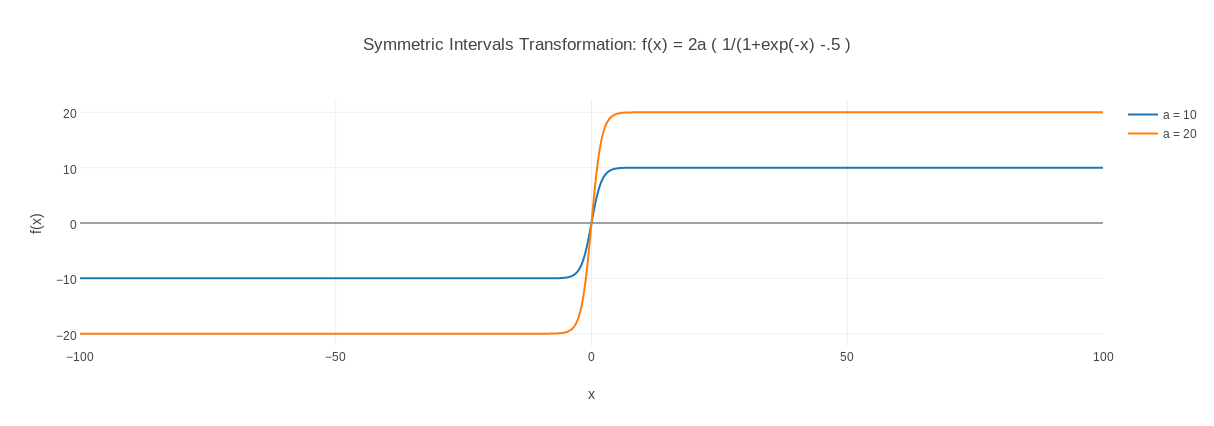
\includegraphics[width=4.5in, height=3.5in]{symmetric_intervals.png}
\end{figure}
\end{center}

\indent This is relevant in the problem at hand. In particular, the estimands $\sigma_{\eta},\sigma_{\epsilon},\sigma_{\eta,\epsilon}$ need to satisfy
\begin{eqnarray}
\sigma_{\eta}^2 \times \sigma_{\epsilon}^2 &>& \sigma_{\eta,\epsilon}^2 \nonumber \\
&=& -\sigma_{\eta} \sigma_{\epsilon} < \sigma_{\eta,\epsilon} < \sigma_{\eta} \sigma_{\epsilon}
\end{eqnarray}

\noindent for the co-variance matrix of $\eta,\epsilon$ to be positive definite. If this restrictions are ignored and the initial conditions are arbitrary (i.e., the researcher ignores how the data generating process behaves and the initial conditions are a guess) the optimization routine may fail to have success. See the codes ``womansestimation.jl'' and ``womandestimation.jl'' to clarify how this works in practice.




\end{document}




